\subsection{UC5 - Impostazioni per Heatmap}
    \label{uc5}
    
    \begin{figure}[htbp]
        \centering
        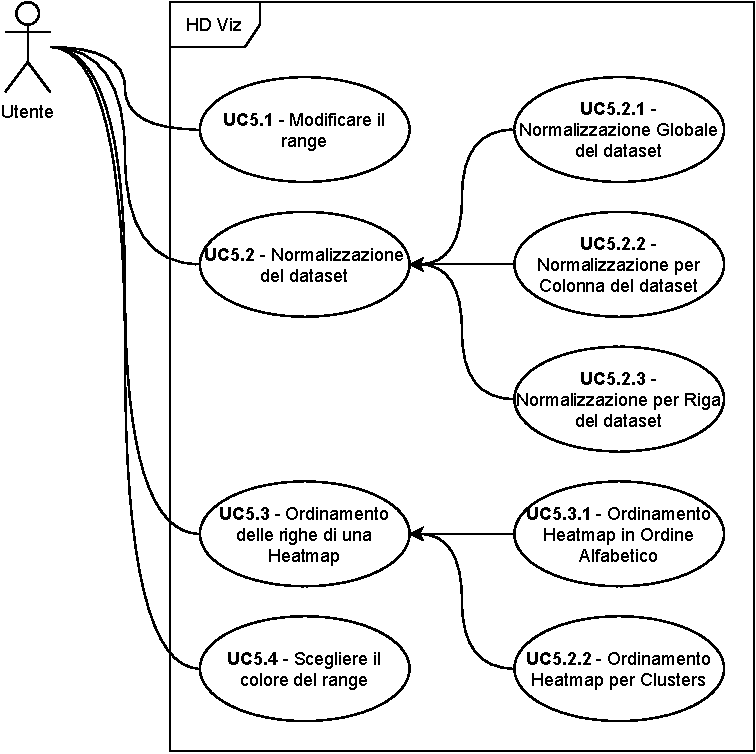
\includegraphics[width=0.7\textwidth]{source/sections/casi-uso/diagrams/uc5.pdf}
        \caption{UC5 - Impostazioni per Heatmap}
        \label{fig:uc5}
    \end{figure}
    
    \begin{itemize}
    \item \textbf{Attore}: Utente
    \item \textbf{Descrizione}: L'utente ha scelto come visualizzazione l'heatmap e regolato le impostazione relative.
    \item \textbf{Precondizione}: 
    \begin{itemize}
        \item Eseguito l'upload del dataset come matrice $N\times M$ (\hyperref[uc1]{UC1}).
        \item Selezionato Heatmap come visualizzazione (\hyperref[uc2.2]{UC2.2}).
    \end{itemize}  
    \item \textbf{Postcondizione}: L'utente ha regolato secondo le proprie necessità le impostazioni relative alla visualizzazione Heatmap
    \item \textbf{Scenario Principale}: 
    \begin{enumerate}
        \item L'utente sceglie se modificare il range della heatmap (\hyperref[uc5.1]{UC5.1})
        \item L'utente sceglie se modificare il colore del range (\hyperref[uc5.4]{UC5.4})
        \item L'utente sceglie se normalizzare il dataset (\hyperref[uc5.2]{UC5.2})
        \item L'utente sceglie se ordinare il dataset (\hyperref[uc5.3]{UC5.3})
    \end{enumerate}  
    \end{itemize}

    \subsubsection{UC5.1 - Modificare il Range}
    \label{uc5.1}
    \begin{itemize}
    \item \textbf{Attore}: Utente
    \item \textbf{Descrizione}: L'utente decide di modificare il range (range di $\textrm{default}=[min, max]$ dove $min=\textrm{valore minimo presente nel dataset}$ e $max=\textrm{valore massimo presente nel dataset}$), su cui ogni valore assume una diversa sfumatura di colore, cioè se viene scelto un range $[min, max-i]$, tutti i valori $\geq max-i$ presenti nel dataset verranno visualizzati con lo stesso colore.
    \item \textbf{Precondizione}: 
    \begin{itemize}
        \item Eseguito l'upload del dataset come matrice $N\times M$ (\hyperref[uc1]{UC1}).
        \item Selezionato Heatmap come visualizzazione (\hyperref[uc2.2]{UC2.2}).
    \end{itemize}  
    \item \textbf{Postcondizione}: Ricolorazione della Heatmap in base al range selezionato: il valore più scuro sarà associato al valore più alto del nuovo range e il valore più chiaro al valore più basso.
    \item \textbf{Scenario Principale}: 
    \begin{enumerate}
        \item L'utente modifica i valori di minimo e massimo su cui il sistema andrà a eseguire la sfumatura del colore
    \end{enumerate}  
    \end{itemize}
    
    
    \subsubsection{UC5.2 - Normalizzazione del dataset}
    \label{uc5.2}
    \begin{itemize}
    \item \textbf{Attore}: Utente
    \item \textbf{Descrizione}: Un dataset può contenere dati non normalizzati, normalizzare il dataset può risultare utile per una migliore visualizzazione dei dati.
    \item \textbf{Precondizione}: 
    \begin{itemize}
        \item Eseguito l'upload del dataset come matrice $N\times M$ (\hyperref[uc1]{UC1}).
        \item Selezionato Heatmap come visualizzazione (\hyperref[uc2.2]{UC2.2}).
    \end{itemize}  
    \item \textbf{Postcondizione}: 
    \item \textbf{Scenario Principale}: Il dataset contenente dati non normalizzati viene normalizzato a seconda del tipo di normalizzazione scelto.
    \begin{enumerate}
        \item L'utente seleziona l'opzione di normalizzazione e specifica quale desidera effettuare.
    \end{enumerate}  
    \item \textbf{Generalizzazioni}: 
     \begin{enumerate}
            \item L'utente sceglie su quale subset di dati effettuare la normalizzazione:
                \begin{enumerate}
                    \item Normalizzazione Globale (\hyperref[uc5.2.1]{UC5.2.1})
                    \item Normalizzazione per Colonna (\hyperref[uc5.2.2]{UC5.2.2})
                    \item Normalizzazione per Riga (\hyperref[uc5.2.3]{UC5.2.3})
                \end{enumerate}
        \end{enumerate}  
    \end{itemize}
    
    \paragraph{UC5.2.1 - Normalizzazione Globale del dataset}
    \label{uc5.2.1}
    \begin{itemize}
    \item \textbf{Attore}: Utente
    \item \textbf{Descrizione}: Un dataset può contenere dati non normalizzati, cioè la media è diversa da 0 o la varianza diversa da 1, normalizzare il dataset può risultare utile per una migliore visualizzazione dei dati.
    In questo caso la normalizzazione viene fatta su tutto il dataset.
    \item \textbf{Precondizione}: 
    \begin{itemize}
        \item Eseguito l'upload del dataset come matrice $N\times M$ (\hyperref[uc1]{UC1}).
        \item Selezionato Heatmap come visualizzazione (\hyperref[uc2.2]{UC2.2}).
    \end{itemize}  
    \item \textbf{Postcondizione}:  Ogni valore ${x_i}_j$ del dataset viene sostituito da $ {y_i}_j = \frac{{x_i}_j - \mu}{\sigma}$ dove $\mu$ è la media dei valori presenti nel data set e $\sigma$ la loro varianza.
    \item \textbf{Scenario Principale}: 
    \begin{enumerate}
        \item L'utente seleziona l'opzione di normalizzazione e specifica che desidera una Normalizzazione Globale.
    \end{enumerate}  
    \end{itemize}
    
    \paragraph{UC5.2.2 - Normalizzazione per Colonna del dataset}
    \label{uc5.2.2}
    \begin{itemize}
    \item \textbf{Attore}: Utente
    \item \textbf{Descrizione}: Un dataset può contenere dati non normalizzati, cioè la media è diversa da 0 o la varianza diversa da 1, normalizzare il dataset può risultare utile per una migliore visualizzazione dei dati.
    In questo caso la normalizzazione viene fatta colonna per colonna.
    \item \textbf{Precondizione}: 
    \begin{itemize}
        \item Eseguito l'upload del dataset come matrice $N\times M$ (\hyperref[uc1]{UC1}).
        \item Selezionato Heatmap come visualizzazione (\hyperref[uc2.2]{UC2.2}).
    \end{itemize}  
    \item \textbf{Postcondizione}: Ogni valore ${x_i}_j$ del dataset viene sostituito da $ {y_i}_j = \frac{{x_i}_j - \mu}{\sigma}$ dove $\mu$ è la media dei valori presenti nella colonna j e $\sigma$ la loro varianza sotto radice.
    \item \textbf{Scenario Principale}: 
    \begin{enumerate}
        \item L'utente seleziona l'opzione di normalizzazione e specifica che desidera una Normalizzazione per Colonna. 
    \end{enumerate}  
    \end{itemize}
    
    \paragraph{UC5.2.3 - Normalizzazione per Riga del dataset}
    \label{uc5.2.3}
    \begin{itemize}
    \item \textbf{Attore}: Utente
    \item \textbf{Descrizione}: Un dataset può contenere dati non normalizzati, cioè la media è diversa da 0 o la varianza diversa da 1, normalizzare il dataset può risultare utile per una migliore visualizzazione dei dati.
    In questo caso la normalizzazione viene fatta riga per riga.
    \item \textbf{Precondizione}: 
    \begin{itemize}
        \item Eseguito l'upload del dataset come matrice $N\times M$ (\hyperref[uc1]{UC1}).
        \item Selezionato Heatmap come visualizzazione (\hyperref[uc2.2]{UC2.2}).
    \end{itemize}  
    \item \textbf{Postcondizione}:  Ogni valore ${x_i}_j$ del dataset viene sostituito da $ {y_i}_j = \frac{{x_i}_j - \mu}{\sigma}$ dove $\mu$ è la media dei valori presenti nella riga i e $\sigma$ la loro varianza sotto radice.
    \item \textbf{Scenario Principale}: 
    \begin{enumerate}
        \item L'utente seleziona l'opzione di normalizzazione e specifica che desidera una Normalizzazione per Riga. 
    \end{enumerate}  
    \end{itemize}
    
    \subsubsection{UC5.3 - Ordinamento delle righe di una Heatmap}
    \label{uc5.3}
  %  \includegraphics{}
    \begin{itemize}
    \item \textbf{Attore}: Utente
    \item \textbf{Descrizione}: L'utente seleziona in che modo organizzare la visualizzazione delle righe di una heatmap, scegliendo tra l'ordine alfabetico o raggruppamento in clusters.
    \item \textbf{Precondizione}: 
    \begin{itemize}
        \item Eseguito l'upload del dataset come matrice $N\times M$ (\hyperref[uc1]{UC1}).
        \item Selezionato Heatmap come visualizzazione (\hyperref[uc2.2]{UC2.2}).
    \end{itemize}  
    \item \textbf{Postcondizione}: Riordinazione della Heatmap in base all'ordinamento selezionato.
    \item \textbf{Scenario Principale}: 
    \begin{enumerate}
        \item L'utente sceglie quale ordinamento desidera effettuare.
    \end{enumerate}  
    \item \textbf{Generalizzazioni}: 
     \begin{enumerate}
            \item L'utente sceglie quale tipo di ordinamento
                \begin{enumerate}
                    \item Ordine Alfabetico (\hyperref[uc10.1]{UC10.1})
                    \item Raggruppamento in Clusters (\hyperref[uc10.2]{UC10.2})
                    \end{enumerate}
        \end{enumerate} 
    \end{itemize}
    
    \paragraph{UC5.3.1 - Ordinamento Heatmap in Ordine Alfabetico}
    \label{uc5.3.1}
    \begin{itemize}
    \item \textbf{Attore}: Utente
    \item \textbf{Descrizione}: Ordinamento delle righe della heatmap in ordine alfabetico.
    \item \textbf{Precondizione}: 
    \begin{itemize}
        \item Eseguito l'upload del dataset come matrice $N\times M$ (\hyperref[uc1]{UC1}).
        \item Selezionato Heatmap come visualizzazione (\hyperref[uc2.2]{UC2.2}).
        \item Selezionata una etichetta di categoria su cui effettuare l'ordinamento.
    \end{itemize}  
    \item \textbf{Postcondizione}: Riordinazione delle righe della Heatmap in ordine alfabetico.
    \item \textbf{Scenario Principale}: 
    \begin{enumerate}
        \item L'utente sceglie di ordinare le righe in ordine alfabetico.
    \end{enumerate}  
    \end{itemize}
    
    \paragraph{UC5.3.2 - Ordinamento Heatmap per Clusters}
    \label{uc5.3.2}
    \begin{itemize}
    \item \textbf{Attore}: Utente
    \item \textbf{Descrizione}: Le righe vengono raggruppate secondo un algoritmo di cluster gerarchico, la distanza calcolata  tra le righe, utilizzata dall'algoritmo, è quella euclidea.
    \item \textbf{Precondizione}: 
    \begin{itemize}
        \item Eseguito l'upload del dataset come matrice $N\times M$ (\hyperref[uc1]{UC1}).
        \item Selezionato Heatmap come visualizzazione (\hyperref[uc2.2]{UC2.2}).
    \end{itemize}  
    \item \textbf{Postcondizione}: Le righe sono raggruppate secondo l'algoritmo di Cluster Gerarchico ed è visualizzato il dendrogramma sviluppato dall'algoritmo.
    \item \textbf{Scenario Principale}: 
    \begin{enumerate}
        \item L'utente sceglie di ordinare le righe tramite clustering.
    \end{enumerate}  
    \end{itemize}
    
        %%%
    \subsubsection{UC5.4 - Assegnare Colore al Range}
    \label{uc5.4}
    
    \begin{itemize}
    \item \textbf{Attore}: Utente
    \item \textbf{Descrizione}: L'utente seleziona il colore ((colori)) con cui vuole evidenziare i valori di una Heatmap,(( la sfumatura più bassa del colore selezionato verrà associata ai valori più bassi e la sfumatura più alta ai valori più alti. ))
    \item \textbf{Precondizione}: 
    \begin{itemize}
        \item Selezionato Heatmap o Correlation Heatmap come visualizzazione (\hyperref[uc2.2]{UC2.2} o \hyperref[uc2.3]{UC2.3})
    \end{itemize}  
    \item \textbf{Postcondizione}: La Heatmap conterrà nelle sue caselle le sfumature del colore selezionato.
    \item \textbf{Scenario Principale}: 
    \begin{enumerate}
        \item L'utente seleziona il colore con cui vuole visualizzare la Heatmap.
    \end{enumerate}  
    \end{itemize}